\documentclass{article}
\usepackage[utf8]{inputenc}
\usepackage[pdftex]{graphicx} %for embedding images
\usepackage{url} %for proper url entries
\usepackage[bookmarks, colorlinks=false, pdfborder={0 0 0}, pdftitle={Project 01 Report: Search On Graph}, pdfauthor={Nhut-Nam Le}, pdfsubject={Fundamentals of Artificial Intelligence}, pdfkeywords={report}]{hyperref} %for creating links in the pdf version and other additional pdf attributes, no effect on the printed document
%\usepackage[final]{pdfpages} %for embedding another pdf, remove if not required
\usepackage[utf8]{vietnam}
\usepackage{booktabs}
\usepackage{float}
\usepackage{smartdiagram}
\usepackage{xcolor}
\usepackage[]{algorithm2e}
\usepackage[noend]{algpseudocode}
\usepackage[]{algorithm}
\usepackage{amsmath}
\usepackage{amsfonts}
\usepackage{nicefrac}
\usepackage{amssymb}
\usepackage{arevmath}     % For math symbols
\usesmartdiagramlibrary{additions}
\usepackage[left=3cm, right=3cm, top=2cm, bottom=2cm]{geometry}
\usepackage{parskip}
\usepackage{tikz}
\usepackage{hyperref}
\setlength{\parindent}{15pt}
\setcounter{secnumdepth}{4}
\newcommand{\ra}[1]{\renewcommand{\arraystretch}{#1}}
\newcommand{\code}[1]{\texttt{#1}}
\newcommand\tab[1][1cm]{\hspace*{#1}}
\usepackage{fancyhdr}

\usepackage{pythonhighlight}

\setlength{\headheight}{15.2pt}
\pagestyle{fancy}
\lhead[<even output>]{Cơ sở trí tuệ nhân tạo}
\rhead[<even output>]{Tìm kiếm trên đồ thị}

\title{report-lab-01-AI}
\author{lenam.fithcmus }
\date{October 2020}

%%% Coloring the comment as blue
\newcommand\mycommfont[1]{\footnotesize\ttfamily\textcolor{blue}{#1}}
\algnewcommand\algorithmicforeach{\textbf{for each}}
\algdef{S}[FOR]{ForEach}[1]{\algorithmicforeach\ #1\ \algorithmicdo}
\newcommand{\LoopDo}{\bf loop do}
\SetCommentSty{mycommfont}

\SetKwInput{KwInput}{Input}                % Set the Input
\SetKwInput{KwOutput}{Output}              % set the Output
\let\oldemptyset\emptyset
\let\emptyset\varnothing

\begin{document}

\begin{titlepage}

\begin{center}

% Top of the page

\includegraphics[width=0.18\textwidth]{hcmus.png}\\[0.1in]
\large{ĐẠI HỌC KHOA HỌC TỰ NHIÊN, ĐHQG-HCM\\KHOA CÔNG NGHỆ THÔNG TIN\\BỘ MÔN KHOA HỌC MÁY TÍNH}\\
\normalsize
\vspace{2cm}
\textup{\large {FUNDAMENTALS OF ARTIFICIAL INTELLIGENCE - CƠ SỞ TRÍ TUỆ NHÂN TẠO} \\ \Large PROJECT REPORT 01 - BÁO CÁO ĐỒ ÁN 01}\\[0.2in]

% Title
\huge \textbf {\\SEARCH ON GRAPH - TÌM KIẾM TRÊN ĐỒ THỊ}\\[0.2in]
\normalsize
\begin{tikzpicture}
  [scale=.8,auto=left,every node/.style={circle,fill=blue!20}]
  \node (n6) at (1,10) {6};
  \node (n4) at (4,8)  {4};
  \node (n5) at (8,9)  {5};
  \node (n1) at (11,8) {1};
  \node (n2) at (9,6)  {2};
  \node (n3) at (5,5)  {3};

  \foreach \from/\to in {n6/n4,n4/n5,n5/n1,n1/n2,n2/n5,n2/n3,n3/n4}
    \draw (\from) -- (\to);

\end{tikzpicture}
\newline
% Submitted by
\normalsize
% Lecturers
Giảng viên lý thuyết\\
{\textbf{GS.TS Lê Hoài Bắc}}\\[0.1in]
% Teacher Assistant
Giảng viên hướng dẫn\\
{\textbf{Dương Nguyễn Thái Bảo, Nguyễn Ngọc Đức, Hoàng Xuân Trường}}\\[0.2in]
Người thực hiện \\
\begin{table}[h]
\centering
\begin{tabular}{lr}\hline \\
Họ và tên: Lê Nhựt Nam\\
Mã số sinh viên: 18120061\\
Email: 18120061@student.hcmus.edu.vn\\
\hline
\end{tabular}
\end{table}
\vspace{0.2in}

% Date time when written report
\vfill
Tháng 10 năm 2020
\end{center}
\end{titlepage}
\newpage
% End Title

\pagenumbering{roman} %numbering before main content starts
\cleardoublepage
%\pagebreak
\phantomsection
\addcontentsline{toc}{section}{Lời cảm ơn}
\section*{Lời cảm ơn}
\vspace{1.0in}
\begingroup
\setlength{\parindent}{0pt}
Trong quá trình thực hiện đồ án này, em đã nhận được rất nhiều sự giúp đỡ cũng như hỗ trợ từ các thầy cô Trường Đại học Khoa học Tự nhiên, ĐHQG-HCM và các bạn bè trong lớp Cơ sở Trí tuệ Nhân tạo. Em xin bày tỏ lòng cảm ơn chân thành đến mọi người vì đã giúp đỡ hướng dẫn, chỉ bảo rất tận tình.

Đặc biệt, em xin bày tỏ lòng biết ơn sâu sắc đến các thầy cô khoa Công nghệ Thông tin, cụ thể hơn là thầy Lê Hoài Bắc và các thầy hướng dẫn đã giảng dạy rất kĩ lưỡng, cung cấp nhiều slides, tài nguyên học tập cần thiết, tạo điều kiện tốt nhất để bản thân em có thể hoàn thành được đồ án này.

Trong quá trình, viết báo cáo này, bản thân em không thể tránh khỏi nhiều sai sót về mặt chuyên môn phân tích thuật toán, nguồn thông tin có thể sai sót và nhất là việc trình bày code có thể chưa hoàn thiện về mặt "clean code", ... Em mong nhận được góp ý để hoàn thiện hơn đối với đồ án này, cũng như rút kinh nghiệm cho những đồ án kế tiếp.
\par


{Đại học Khoa học Tự nhiên, ĐHQG-HCM.}\\
Lê Nhựt Nam\\
Tháng 10 năm 2020,\\
\endgroup

\newpage
\tableofcontents
\newpage
\pagenumbering{arabic} %reset numbering to normal for the main content

\section{Tổng quan về đồ án}
\subsection{Mục tiêu của đồ án}
\setlength{\parindent}{10ex}
Nghiên cứu, cài đặt và trình bày các thuật toán tìm kiếm trên đồ thị


\subsection{Các yêu cầu}
\begin{itemize}
	\item Thông tin sinh viên: họ tên, MSSV…
	\item Mức độ hoàn thành của mỗi mức yêu cầu. Tự đánh giá đồ án trên thang điểm 10.
	\item Trình bày lý thuyết cơ bản (ý tưởng, độ phức tạp, tính chất,...) của mỗi thuật toán cài đặt (BFS, DFS, UCS, $A^{*}$).
	\item Trình bày điểm khác biệt giữa UCS và A*.
	\item Thuật toán tìm kiếm khác ngoài 4 thuật toán (BFS, DFS, UCS, $A^{*}$): Greedy Best-First Search
\end{itemize}

\subsection{Bảng tự đánh giá mức độ hoàn thành công việc}

\begin{table*}[h]\centering
\ra{1.3}
\begin{tabular}{lllll}\toprule
\textbf{STT} & \textbf{Tiêu chí} & \textbf{Mức độ} & \textbf{Điểm} & \textbf{Ghi chú} \\\midrule
1 & Trình bày thuật toán BFS & 100\% & 10 & \\
2 & Trình bày thuật toán DFS & 100\% & 10 & \\
3 & Trình bày thuật toán UCS & 100\% & 10 & \\
4 & Trình bày thuật giải A* & 100\% & 10 & \\
5 & Trình bày các sinh trọng số để chạy UCS và A* & 100\% & 10 & \\
6 & Trình thuật toán Greedy Best-First Search & 100\% & 10 & Điểm cộng\\
7 & Trình bày điểm khác biệt giữa UCS và A* & 100\% & 10 & \\
8 & Chạy thử và có video demo (Ít nhất 3 testcase) cho mỗi thuật toán & 100\% & 10 & \\
9 & Có trình bày báo cáo & 100\% & 10 & \\
\bottomrule
\end{tabular}
\end{table*}

\newpage

\section{Lý thuyết cơ bản}

\subsection{Thuật toán tìm kiếm theo chiều rộng - Breadth First Search}

Thuật toán Breadth First Search (BFS - Tìm kiếm theo chiều rộng) là thuật toán xét (duyệt) hoặc tìm kiếm trên cây và đồ thị, có chiến lược tìm kiếm mù (tìm kiếm không có định hướng, không chú ý đến thông tin, giá trị được duyệt).\newline

\subsubsection{Ý tưởng}
Thuật toán có chiến lược tìm kiếm đơn giản bằng việc xây dựng cây tìm kiếm theo chiều rộng, nút gốc được mở rộng đầu tiên, sau đó tất cả những nút con của nút gốc sẽ được mở rộng, tiếp theo và tiếp sau các nút con của những nút con đó sẽ được mở rộng. \newline
Tổng quát: Tất cả các nút ở độ sâu d trong cây tìm kiếm sẽ được mở rộng trước những nút ở độ sâu d + 1

\begin{figure}[h]
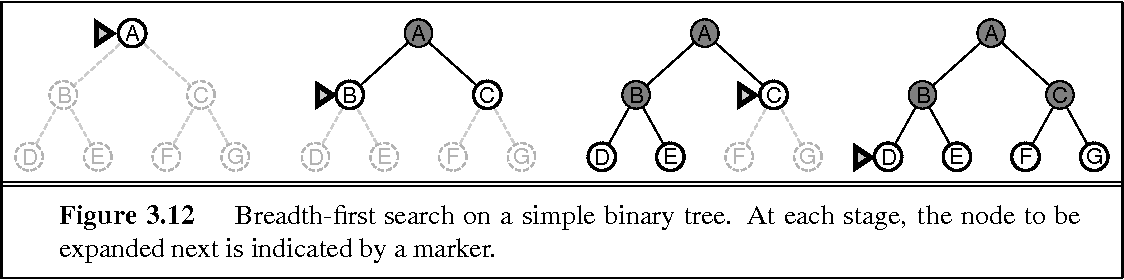
\includegraphics[width=16cm]{19-Figure3.12-1.png}
\centering
\end{figure}

\subsubsection{Mã giả - Pseudocode}

\begin{algorithm}[H]
\DontPrintSemicolon
  
\KwInput{Bài toán/ Vấn đề, Ngăn chứa (FIFO queue)}
\KwOutput{Lời giải cho bài toán hoặc không có lời giải (Thất bại)}
\KwData{Testing set $x$}
\Function{Breadth-First-Search}{problem} 
\Return{a solution, or failure}

node $\leftarrow$ a node with State = problem.Initial-State, Path-Cost = 0 \\
\If{problem.Goal-Test(node.State)}
{
    \Return{Solution(node)}
}

frontier $\leftarrow$ node\\
explored $\leftarrow$ $\oldemptyset$\\
\LoopDo\\
\If{frontier = $\oldemptyset$}
{
 \Return{Failure}
}
node $\leftarrow$ Pop(frontier)\\
add node.State to explored \\
\ForEach{action {\bf in} problem.Actions(node.State)}
{
    child $\leftarrow$ Child-Node(problem, node, action)
    
    \If{child.State {\bf is not in} explored  {\bf or} frontier}
    {
        \If{problem.Goal-Test(child.State)}
        {
            \Return{Solution(child)}
        }
        frontier $\leftarrow$  Insert(child, frontier)
    }
}
\EndFunction
\caption{Thuật toán tìm kiếm theo chiều rộng - Breadth-First Search Algorithm (Artificial Intelligence: A Modern Approach (3rd Edition) - Breadth-First Search Pseudocode) - P82}
\end{algorithm}

\subsubsection{Đánh giá thuật toán}
Đầu vào tìm kiếm theo chiều rộng được giả định là một đồ thị hữu hạn, được biểu diễn một cách rõ ràng dưới dạng danh sách kề, ma trận kề hoặc biểu diễn tương tự .Nhưng trong lý thuyết, ta phải ngầm định rằng đầu vào có thể là một biểu diễn ngầm định của một đồ thị vô hạn.

\paragraph{Tính đầy đủ}
Breadth-First Search có tính đã đầy đủ - nếu nút mục tiêu nông nhất ở độ sâu d, nó cuối cùng sẽ tìm thấy nó sau khi mở rộng tất cả các nút nông hơn d.
\paragraph{Tính tối ưu}
Breadth-First Search dừng lại ở mục tiêu nông nhất được tìm thấy, mục tiêu nông nhất này có thể không nhất thiết là tối ưu nhất. Nên trường hợp tổng quát, nó sẽ không tối ưu
\paragraph{Độ phức tạp về thời gian}
Với $b$ là số nút con của những nút không phải đích đến, $d$ là độ sâu khi tìm thấy đích.\\
Ta có độ phức tạp thuật toán: $1 + b^1 + b^2 + b^3 + ... + b^d = O(b^d)$
\paragraph{Độ phức tạp về không gian}
Với $b$ là số nút con của những nút không phải đích đến, $d$ là độ sâu khi tìm thấy đích.\\
Tất cả các trạng thái phải được ghi nhớ để tránh các đường dẫn dư thừa và lặp lại. Do đó, cho đến khi đạt đến nút mục tiêu ở độ sâu $d$, tất cả các nút cho đế n$d-1$ phải được lưu trong bộ nhớ.
Ta có độ phức tạp về không gian: $b^1 + b^2 + b^3 + ... + b^d = O(b^d)$ ($ O(b^{d-1)}$ cho những đỉnh đã được duyệt lưu trong explored và  $O(b^{d})$ cho hàng đợi)
\subsection{Thuật toán tìm kiếm theo chiều sâu - Depth First Search}

\subsubsection{Ý tưởng}
Thuật toán bắt đầu ở nút gốc (chọn một số nút tùy ý làm nút gốc trong trường hợp biểu đồ) và khám phá càng xa càng tốt dọc theo mỗi nhánh trước khi backtracking.

\begin{figure}[H]
\centering
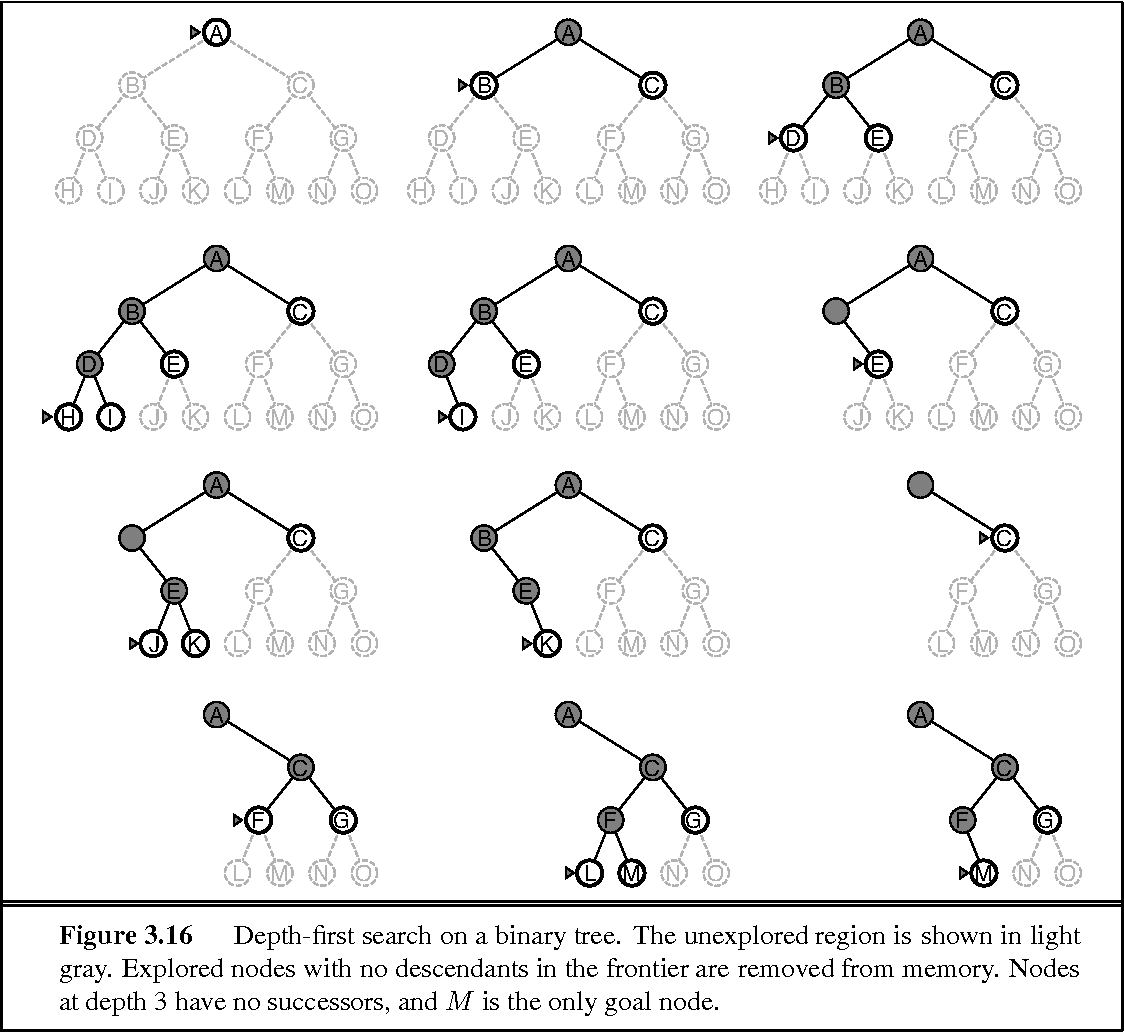
\includegraphics[width=0.5\textwidth]{23-Figure3.16-1.png}
\caption{Artificial Intelligence: A Modern Approach (3rd Edition) Depth First Search}
\end{figure}

\subsubsection{Đánh giá thuật toán}
Đầu vào DFS được giả định là một đồ thị hữu hạn, được biểu diễn một cách rõ ràng dưới dạng danh sách kề, ma trận kề hoặc biểu diễn tương tự .Nhưng trong lý thuyết, ta phải ngầm định rằng đầu vào có thể là một biểu diễn ngầm định của một đồ thị vô hạn.

\paragraph{Tính đầy đủ: }
Thuật toán DFS không đảm bảo tính đầy đủ nếu không gian tìm kiếm là vô hạn, khi không gian tìm kiếm hữu hạn thì ngược lại.

\paragraph{Tính tối ưu: }
Thuật toán DFS không đảm bảo tính tối ưu

\paragraph{Độ phức tạp về thời gian}
Tăng theo hàm mũ $O(b^m)$, xấu là khi m lớn hơn nhiều lần so với độ sâu d, tốt nhất khi lời giải không ở quá sâu
\paragraph{Độ phức tạp về không gian}
Gần như là tuyến tính $O(bm)$
\subsubsection{Mã giả - Pseudocode thuật toán DFS có giới hạn}
Dựa trên cơ sở của DFS, nhưng có một giới hạn về độ sâu để tránh khỏi rơi vào vòng lặp vô hạn, các nút con của các nút ở độ sâu L có thể coi là không có con.

\begin{figure}[H]
\centering
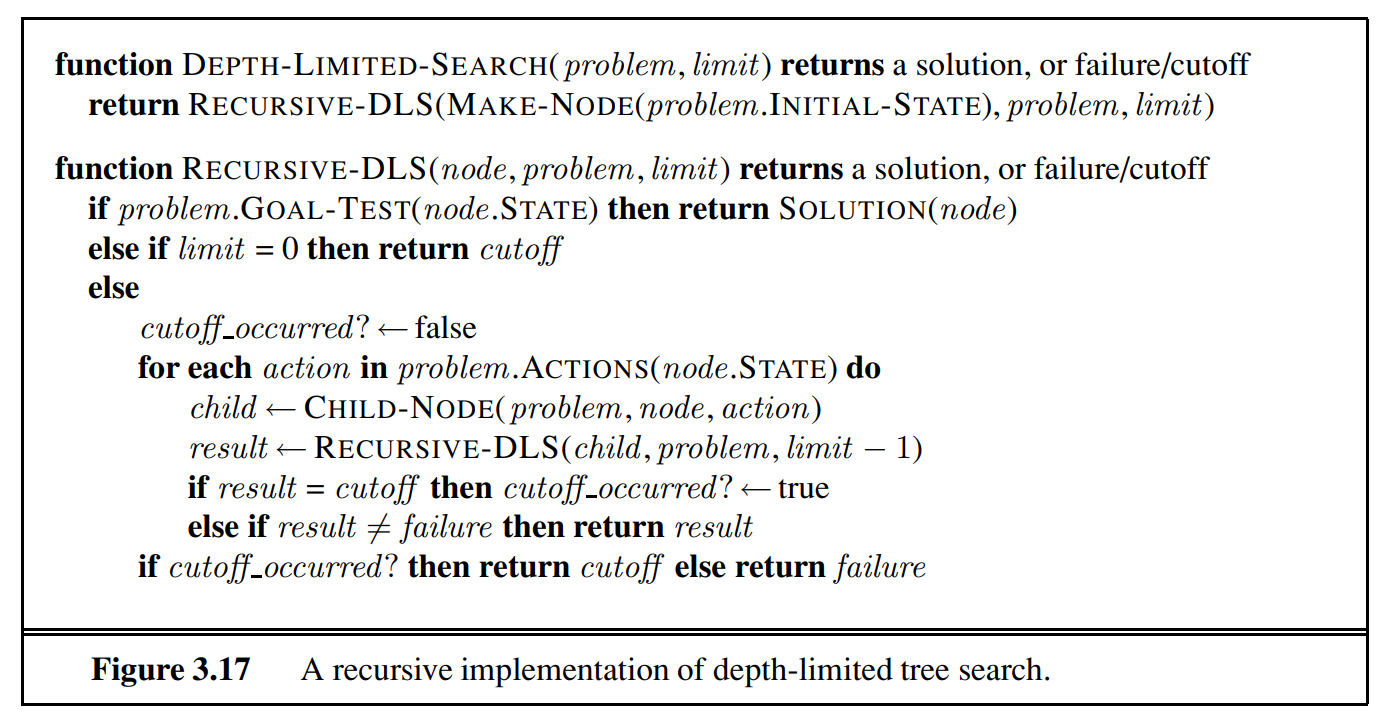
\includegraphics[width=0.98\textwidth]{depth-limit-search-figure-3.17.png}
\caption{Artificial Intelligence: A Modern Approach (3rd Edition) Depth Limit Search Pseudocode}
\end{figure}

Đánh giá:\newline
\begin{itemize}
\item Tính đầy đủ: Nếu L < d thì thuật toán có tính đầy đủ
\item Tính tối ưu: Nếu L < d thì thuật toán có tính tối ưu và không có khi L > d
\item Độ phức tạp về thời gian: $O(b^L)$
\item Độ phức tạp về không gian: $O(bL)$

\end{itemize}

\subsection{Thuật toán tìm kiếm đồng nhất - Uniform Cost Search}

\subsubsection{Hàng đợi ưu tiên - Priority Queue}
Hàng đợi ưu tiên là một cấu trúc dữ liệu trong đó ta có thể thêm và lấy ra các phần tử dựa trên độ ưu tiên của mỗi phần tử. \\
Trong bài lab này, sử dụng module queue với class PriorityQueue của Python, các thao tác thêm và lấy đều có độ phức tạp là $O(logN)$ với $N$ là số phần tử trong hàng đợi ưu tiên.

\subsubsection{Hàm chi phí - Cost Function}
Ta có hàm tính chi phí:\\
f(n) = tổng chi phí đường đi từ nút start đến nút n\\
Đối với lab, khoảng cách Euclidean cho ta khoảng cách ngắn nhất trong các loại khoảng cách giữa hai điểm trong toán học nên sẽ dùng khoảng cách này để tính trọng số giữa 2 đỉnh trong đồ thị

\subsubsection{Ý tưởng}

\subsubsection{Mã giả - Pseudocode}
\begin{algorithm}[H]
\DontPrintSemicolon
  
\KwInput{Bài toán/ Vấn đề, Ngăn chứa (FIFO queue)}
\KwOutput{Lời giải cho bài toán hoặc không có lời giải (Thất bại)}
% \KwData{Testing set $x$}
Frontier is a priority queue \\
\Function{Uniform-Cost-Search}{(problem} 
\Return{a solution, or failure}

node $\leftarrow$ a node with State = problem.Initial-State, Path-Cost = 0

frontier $\leftarrow$ node \tcc{a priority queue ordered by Path-Cost}
explored $\leftarrow$ $\oldemptyset$\\
\LoopDo \\
\If{frontier = $\oldemptyset$}
{
 \Return{Failure}
}
node $\leftarrow$ Pop(frontier) \tcc{chooses the lowest-cost node in frontier} \\
\If{problem.Goal-Test(node.State)}
{
    \Return{Solution(node)}
}

add node.State to explored \\
\ForEach{action {\bf in} problem.Actions(node.State)}
{
    child $\leftarrow$ Child-Node(problem, node, action)
    
    \If{child.State {\bf is not in} explored  {\bf or} frontier}
    {
        frontier $\leftarrow$  Insert(child, frontier)
    }
    \ElseIf{child.State {\bfis in} explored {\bf with} higher Path-Cost} 
    {
        replace that frontier node with child
    }
}
\EndFunction

\caption{Thuật toán chi phí đồng nhất - Uniform-cost Search Algorithm (Artificial Intelligence: A Modern Approach (3rd Edition) - Uniform-cost Search Pseudocode) - P84}
\end{algorithm}


\subsubsection{Đánh giá thuật toán}
Đầu vào tìm kiếm tìm kiếm đồng nhất được giả định là một đồ thị hữu hạn, được biểu diễn một cách rõ ràng dưới dạng danh sách kề, ma trận kề hoặc biểu diễn tương tự .Nhưng trong lý thuyết, ta phải ngầm định rằng đầu vào có thể là một biểu diễn ngầm định của một đồ thị vô hạn.

Đánh giá chung:
\begin{itemize}
\item Thuộc loại tìm kiếm mù (không có thông tin) và có thể đưa ra giải pháp tối ưu cho bài toán và khá tương tự với Heuristic Search khi mà hàm h(n) = 0 (một hàm hằng, bằng 0).
\item Với UCS, chắc chắn sẽ tìm thấy lời giải (đường đi) nếu bài toán tồn tại lời giải và đường đi (lời giải) đó là đường đi (lời giải) tốt nhất.
\item Tuy nhiên, điểm yếu của thuật toán này là tốn nhiều không gian lưu trữ và nó có thể bị mắc kẹt trong một vòng lặp vô hạn vì nó xem xét mọi con đường có thể đi từ nút gốc (trạng thái bắt đầu) đến nút đích(trạng thái kết thúc).
\end{itemize}
\paragraph{Tính đầy đủ}
Nếu chi phí giữa mỗi đỉnh là một hằng số dương thì tính đầy đủ của thuật toán tìm kiếm chi phí đồng nhất sẽ được đảm bảo.

\paragraph{Tính tối ưu}
Thuật toán đảm bảo được tính tối ưu, vì ở mỗi bước, đường dẫn với chi phí thấp nhất được chọn và đường dẫn không bao giờ ngắn hơn khi các nút được thêm vào, đảm bảo rằng tìm kiếm mở rộng các nút theo thứ tự chi phí đường dẫn tối ưu của chúng.

\paragraph{Độ phức tạp về thời gian}
Với $b$ là số nút con của những nút không phải đích đến.\\
Với $C^{*}$ là là chi phí đường đi tối ưu của lời giải và mỗi bước tiêu tốn chi phí ít nhất là $e$. Thuật toán có độ phức tạp về thời gian là: \\
$$O(b^{1 + [\frac{C*}{e}]})$$

\paragraph{Độ phức tạp về không gian}
Với $b$ là số nút con của những nút không phải đích đến.\\
Với $C^{*}$ là là chi phí đường đi tối ưu của lời giải và mỗi bước tiêu tốn chi phí ít nhất là $e$. Thuật toán có độ phức tạp về không gian là: \\
$$O(b^{1 + [\frac{C*}{e}]})$$

\subsection{Tìm kiếm $A^{*}$ - $A^{*}$ Search}

Heuristic là phương pháp giải quyết vấn đề dựa trên phỏng đoán, ước chừng, kinh nghiệm, trực giác để tìm ra giải pháp gần như là tốt nhất và nhanh chóng.\newline
Hàm Heuristic là hàm ứng với mỗi trạng thái hay mỗi sự lựa chọn một giá trị ý nghĩa đối với vấn đề dựa vào giá trị hàm này ta lựa chọn hành động.\newline
Tìm kiếm $A^{*}$ (Đọc là: a star) là mộ hình thức của tìm kiếm tối ưu (Best-First Search) được biết đến nhiều nhất  \newline
$A^{*}$ là một thuật giải đánh giá một nút dựa trên chi phí từ nút gốc đến nút đó - $g(n)$ cộng với một ước lượng chi phí từ nút đó đến đích - $h(n)$ \newline
Evaluation function:
$$f(n) = g(n) + h(n)$$
Trong đó:\newline
- $g(n)$ là chi phí từ nút gốc đến nút n hiện tại.\newline
- $h(n)$ là ước lượng chi phí ngắn nhất để đi từ nút hiện tại n đến đích.\newline
- $f(n)$ là ước lượng chi phí của lời giải "tốt nhất" qua n.\newline
\newline
Trường hợp đặc biệt của $A^{*}$
\newline
Trường hợp hàm đánh giá (Evaluation function) của chúng ta là:
$$f(n) = g(n)$$
Đó là Uniform-Cost Search (Tìm kiếm với chi phí đồng nhất với các thông tin đỉnh, cung, giá thành cung, thực hiện trên cây. $\Longrightarrow$ $A^{T}$
\newline
Trường hợp hàm đánh giá (Evaluation function) của chúng ta là:
$$f(n) = h(n)$$
Đó là tìm kiếm tham lam Heuristic với các thông tin đỉnh, cung, giá thành cung, tri thức bổ sung từ hàm $h(n)$, thực hiện trên cây. $\Longrightarrow$ $A^{KT}$


\subsubsection{Ý tưởng}
Thuật giải A* cân bằng lại trọng số cho đồ thị và sâu đó tìm kiếm bằng thuật toán Dijsktra (có thể thay bằng những thuật toán khác) trên đồ thị mới này, giảm thiểu số nút phải mở ra\newline
Chọn hàm Heuristic đối với lab:\newline
Python code cho một số công thức khoảng cách toán học:\newline
\begin{python}
def euclidean_distance(current_x, current_y, goal_x, goal_y):
    """
    Euclidean distance
    current_node(current_x, current_y)
    goal_node(goal_x, goal_y)
    """
    distance = math.sqrt((goal_x - current_x)**2 + (goal_y - current_y)**2)
    return distance
\end{python}
Khoảng cách Euclidean cho ta khoảng cách ngắn nhất trong các loại khoảng cách giữa hai điểm trong toán học do nó chính là chiều dài của đoạn thẳng nổi hai điểm, hướng mở rộng đường đi của vật thể cũng không bị giới hạn. Đây cũng là Heuristic đơn giản nhất. Nhưng nó gây phức tạp hơn khi phải tính toán bình phương và lấy căn bậc hai, trong khi đồ thị của chúng ta biểu diễn trên khung hình PyGame với tọa độ nguyên. 

\begin{python}
def diagonal_distance(current_x, current_y, goal_x, goal_y):
    """
    Diagonal distance
    current_node(current_x, current_y)
    goal_node(goal_x, goal_y)
    """
    return max(abs(current_x - goal_x),  abs(current_y - goal_y))
\end{python}

\begin{python}
def manhattan_distance(current_x, current_y, goal_x, goal_y):
    """
    Manhattan distance
    current_node(current_x, current_y)
    goal_node(goal_x, goal_y)
    """
    return abs(current_x - goal_x) + abs(current_y - goal_y)
\end{python}
Khoảng cách Manhattan và Diagonal đơn giản hơn, vì lược giản được bình phương và căn bậc hai, trong đó Manhattan cho ta hàm heuristic có giá trị nhỏ hơn. Nên trong bài lab sử dụng khoảng cách Manhattan


\subsubsection{Mã giả - Pseudocode}
Thuật giải A*:\newline
Input: Đồ thị, trạng thái bắt đầu, trạng thái đích đến, hàm heuristic\newline
Output: Lời giải (Đường đi) or thất bại tìm kiếm\newline
Bước 1:
\begin{itemize}
    \item Khởi tạo hai tập rỗng open set và explored set
    \item Đưa trạng thái bắt đầu vào open set
\end{itemize}
Bước 2: \newline
Khởi tạo vòng lặp trong khi open set vẫn chưa rỗng:\newline
- Pop open set, lấy giá trị đỉnh trên đầu open set ra (đây là đỉnh có cost nhỏ nhất) được current node\newline
- Nếu đỉnh này là goal thì trả về path và dừng thuật toán\newline
- neighbors := những đỉnh kề với  current node\newline
- Khởi tạo vòng lặp với mỗi neighbor trong tập neighbors trên:\newline
\tab Nếu neighbor chưa nằm trong tập explored và không xuất hiện trong open set: Đưa neighbor vào explored, tính f = g + h, giá trị new cost := f, đưa neighbor vào open set với path và chi phí đó. Lặp lại bước 2.\newline
\tab Nếu neighbor xuất hiện trong open set: loại bỏ neighbor trong open set, tính f = g + h, giá trị new cost := f, đưa neighbor vào open set với path và chi phí đó. Lặp lại bước 2\newline
Bước 3: Nếu ra khỏi vòng lặp mà chưa có đường di thì trả về thất bại cho bài toán


\subsubsection{Đánh giá thuật toán}
Đánh giá chung:\newline
- Với $A^{*}$ chắc chắn sẽ tìm được đường đi, nếu bài toán có tồn tại lời giải (đường đi) nhưng đường đi này không nhất thiết phải là đường đi tốt nhất do phụ thuộc vào hàm Heuristic.\newline
- Bài toán có tìm được lời giải tối ưu được hay không là do cách chọn hàm Heuristic (Hàm Heuristic ở đây có thể có tính chất admissible heuristic, consistent heuristic). Khi hàm Heuristic chấp nhận được thì Tìm kiếm A* đầy đủ và tối ưu.\newline
\begin{itemize}
\item Heuristic được tính chính xác từ trước: Dựa vào thông tin ước lượng khoảng cách từ cơ sở dữ liệu, data center mà tính toán ra được (Thường không hợp lý lắm vì rất nhiều vấn đề mà con người vẫn chưa thể lưu trữ được hết xuống cơ sở dữ liệu)\newline
\item Heuristic dựa trên tri thức và kinh nghiệm: tri thức toán học về khoảng cách giữa hai điểm cho trước (với giả thiết là không có vật cản chắn giữa đường đi) như: Khoảng cách Manhattan, khoảng cách Chebyshev, khoảng cách Euclid, khoảng cách Diagonal, ...; tri thức về hướng, khoảng cách ước lượng nhờ tính theo đường chim bay, kinh nghiệm đời sống; ...\newline
\end{itemize}
- Yếu điểm của thuật giải: Tốn không gian lưu trữ, vì cần lưu trữ nhiều các tập open set, explored set, path

\paragraph{Tính đầy đủ và tối ưu}
Thuật giải $A^{*}$ sẽ cho ra kết quả đầy đủ và tối ưu nếu hàm heuristic $h(n)$ thỏa một số điều kiện nhất định (Phụ thuộc vào cách chọn hàm heuristic).\newline
Với đồ thị hữu hạn, trọng số không âm, $A^{*}$ đảm bảo được sự kết thúc và đầy đủ, tức là nó sẽ cho ra được lời giải (đường đi từ trạng thái bắt đầu đến trạng thái đích) nếu tồn tại.\newline
Với đồ thị vô hạn, hệ số phân nhánh của mỗi nút hữu hạn và chi phí mỗi cạnh là một số dương, thuật giải vẫn có thể đưa ra được lời giải (đường đi từ trạng thái bắt đầu đến trạng thái đích) nếu tồn tại.

\paragraph{Độ phức tạp về thời gian}
Độ phức tạp về thời gian của A* phụ thuộc vào cách chọn hàm Heuristic hay chính là h(n). Hàm Heuristic tốt và tối ưu thì thuật toán đạt hiệu năng cao.Trong trường hợp xấu nhất của không gian tìm kiếm không bị giới hạn, số lượng nút được mở rộng là cấp số nhân theo chiều sâu d của lời giải (đường đi ngắn nhất): $O(b^{d})$, trong đó b là hệ số phân nhánh
\paragraph{Độ phức tạp về không gian}
Độ phức tạp về không gian của A* gần giống như các thuật toán khác, vì tất cả mọi thứ như đường đi, chi phí cần được lưu trữ, và việc tính toán các hàm heuristic cũng phức tạp, nên sẽ rất tốn bộ nhớ.
\subsection{Tìm kiếm tối ưu kiểu tham lam - Greedy Best First Search}

\subsubsection{Ý tưởng}
Tìm kiếm tối ưu kiểm tham lam mở rộng nút gần đích nhất với hi vọng cách làm này sẽ dẫn đến một lời giải một cách nhanh nhất. Lời giải trên nếu tồn tại có thể không là một lời giải "tốt nhất"\newline
Đánh giá các trạng thại thông qua hàm Heuristic
$$f(n) = h(n)$$
Ta thấy, đây là một trường hợp của A* khi hàm g(n) = 0 (hằng 0)

\subsubsection{Đánh giá thuật toán}

\paragraph{Tính hoàn và tối ưu}
Vì đánh giá dựa vào hàm Heuristic nên ta sẽ tìm được lời giải cho bài toán, lời giải này không nhất thiết phải là một lời giải tốt nhất (hay một đường đi ngắn nhất), nó cố gắng mở rộng nút gần nhất với mục tiêu, với lý do rằng điều này có khả năng dẫn đến một giải pháp nhanh chóng nên nó không hoàn chỉnh và tối ưu [According to the book Artificial Intelligence: A Modern Approach (3rd edition), by Stuart Russel and Peter Norvig, specifically, section 3.5.1 Greedy best-first search (p. 92)]

\paragraph{Độ phức tạp về thời gian}
Khi hàm đánh giá chính là hàm Heuristic, nó phụ thuộc vào cách chọn hàm Heuristic hay chính là h(n). Hàm Heuristic tốt và tối ưu thì thuật toán đạt hiệu năng cao, và nó sẽ gần giống với BFS
\paragraph{Độ phức tạp về không gian}
Khá tương tự với độ phức tạp về không gian của thuật giải A*.
\newpage

\section{Hai thuật toán UCS và $A^{*}$}
Bảng so so sánh sự khác biệt giữa hai thuật toán
\begin{center}
    \begin{tabular}{ | l | p{5cm} | p{5cm} |}
    \hline
    Tiêu chí đánh giá & Uniform-cost Search & A* Search\\ \hline
    Chiến lược & Sử dụng chiến lược tìm kiếm mù (không có thông tin), không có hàm đánh giá (tương tự như A* khi hàm h(n) = 0) & Sử dụng chiến lược tìm kiếm m có thông tin (kinh nghiệm), có sử dụng hàm đánh giá (f(n) = g(n) + h(n) \\ \hline
    Chi phí & Được tính từ trạng thái bắt đầu đến trạng thái hiện tại & Tổng hai chi phí đi từ trạng thái gốc đến trạng thái hiện tại và một ước lượng chi phí từ trạng thái hiện tại đến trạng thái đích  \\ \hline
    Độ phức tạp theo thời gian & $$O(b^{1 + [\frac{C*}{e}]})$$ & $$O(|E|) = O(b^{d})$$  \\\hline
    Độ phức tạp theo không gian & $$O(b^{1 + [\frac{C*}{e}]})$$  & $$O(|E|) = O(b^{d})$$ \\\hline
    Danh sách các node chờ duyệt & Hàng đợi ưu tiên & Hàng đợi ưu tiên \\\hline
    Khả năng tìm nghiệm & Có nhưng một vài trường hợp bị vướng vòng lặp vô hạn & Có thể đưa ra nghiệm tốt \\\hline
    Tối ưu & Có vì chắc chắn tìm được lời giải tốt nhất nếu có tồn tại lời giải & Tìm đường lời giải tốt không nhất thiết phải là lời giải tốt nhất  \\\hline
    \end{tabular}
    
\begin{figure}[H]
\centering

\includegraphics[width=0.5\textwidth]{ucs.png}
\caption{Uniform Cost Search}
\end{figure}

\begin{figure}[H]
\centering
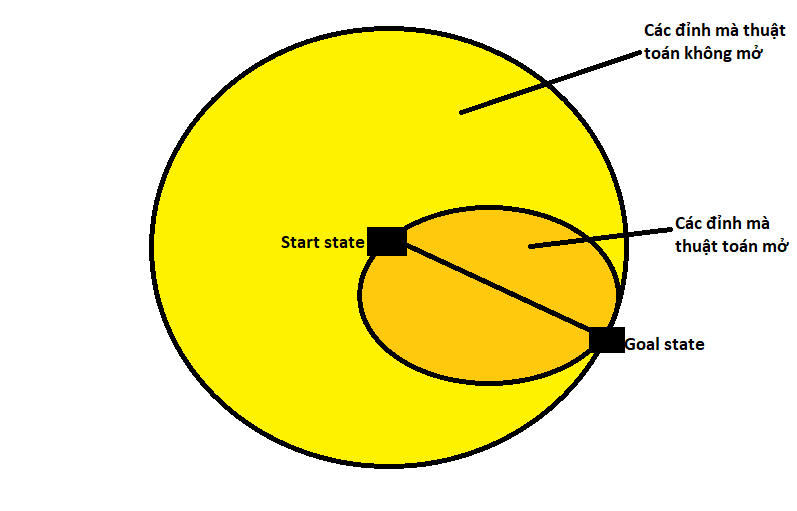
\includegraphics[width=0.5\textwidth]{heuristic.png}
\caption{A* Search}
\end{figure}
\end{center}
\newpage

\section{Demo lab với các testcase}
\subsection{Test case}
\subsubsection{Test case khi lúc nhận đồ án}
\begin{figure}[H]
\centering
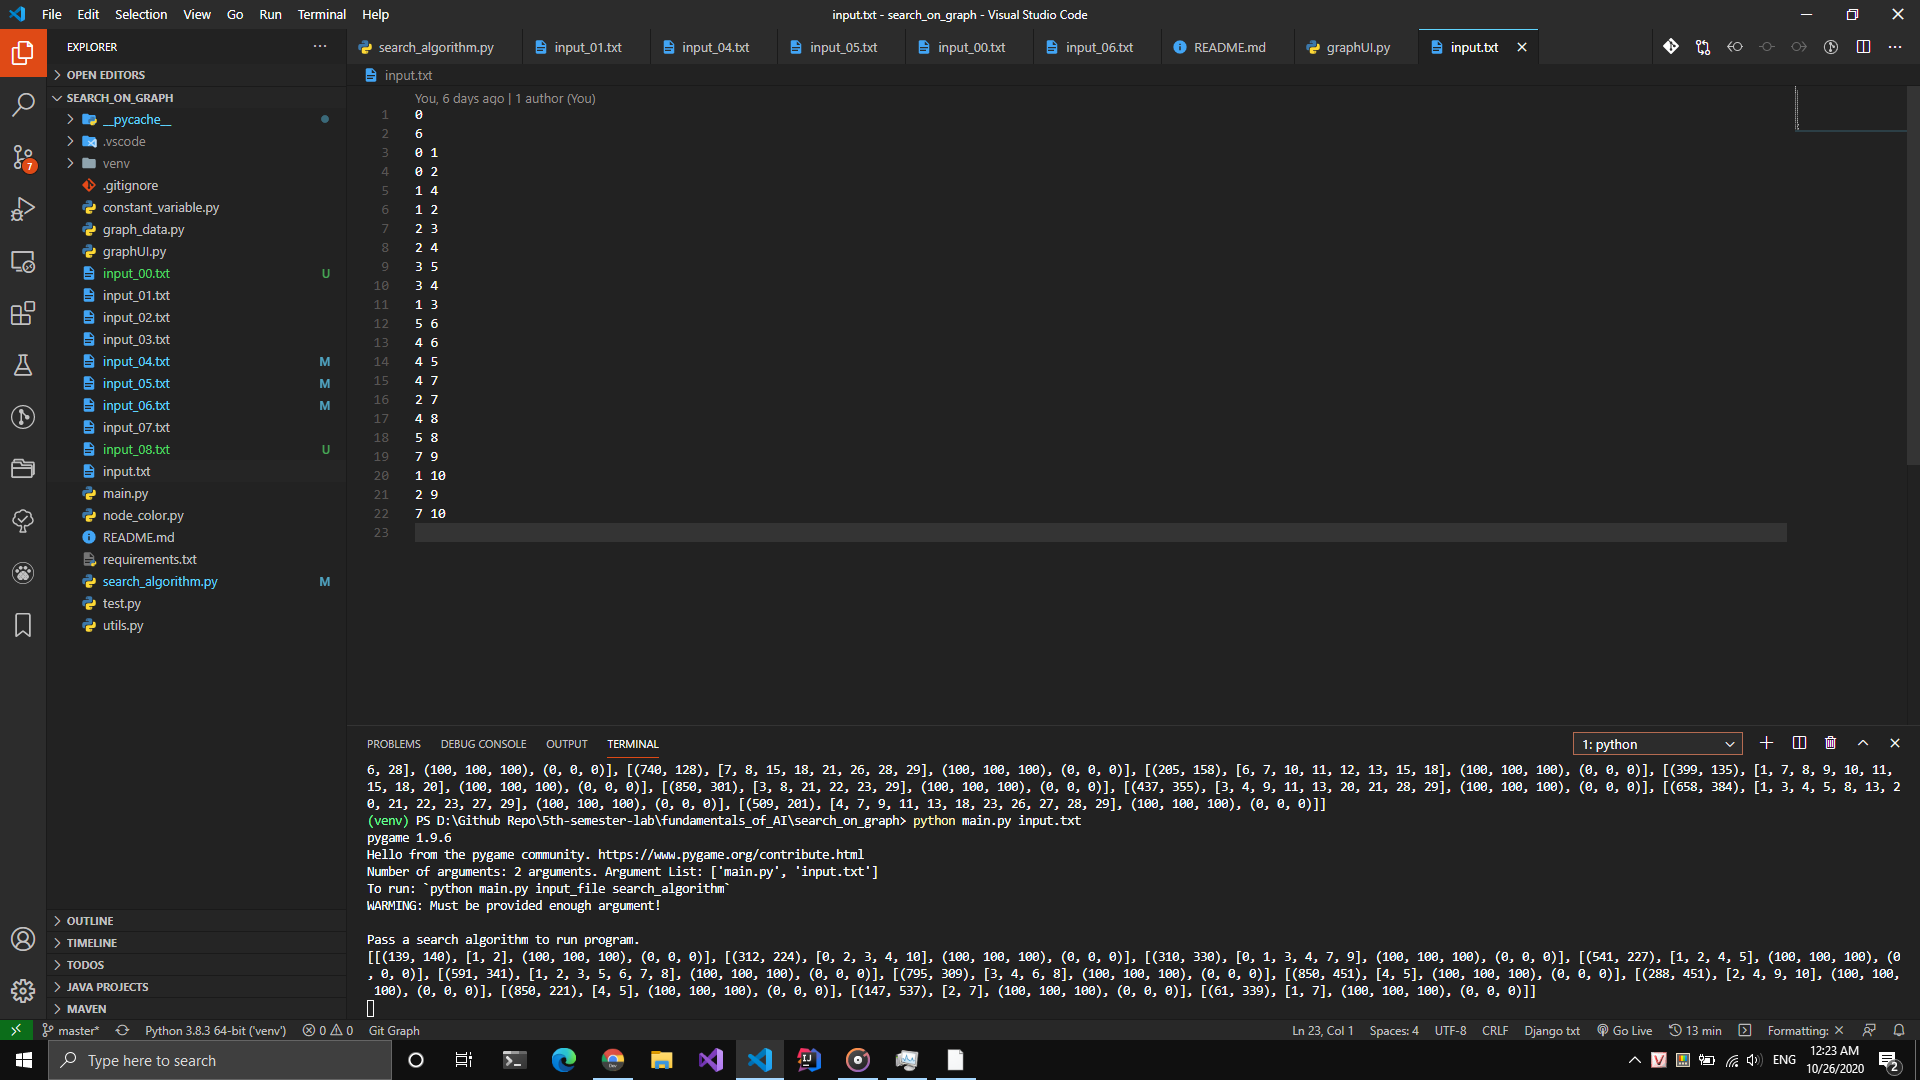
\includegraphics[width=0.5\textwidth]{Test_Case_00.png}
\caption{Testcase mẫu - Kích thước 11 đỉnh}
\end{figure}
\begin{figure}[H]
\centering
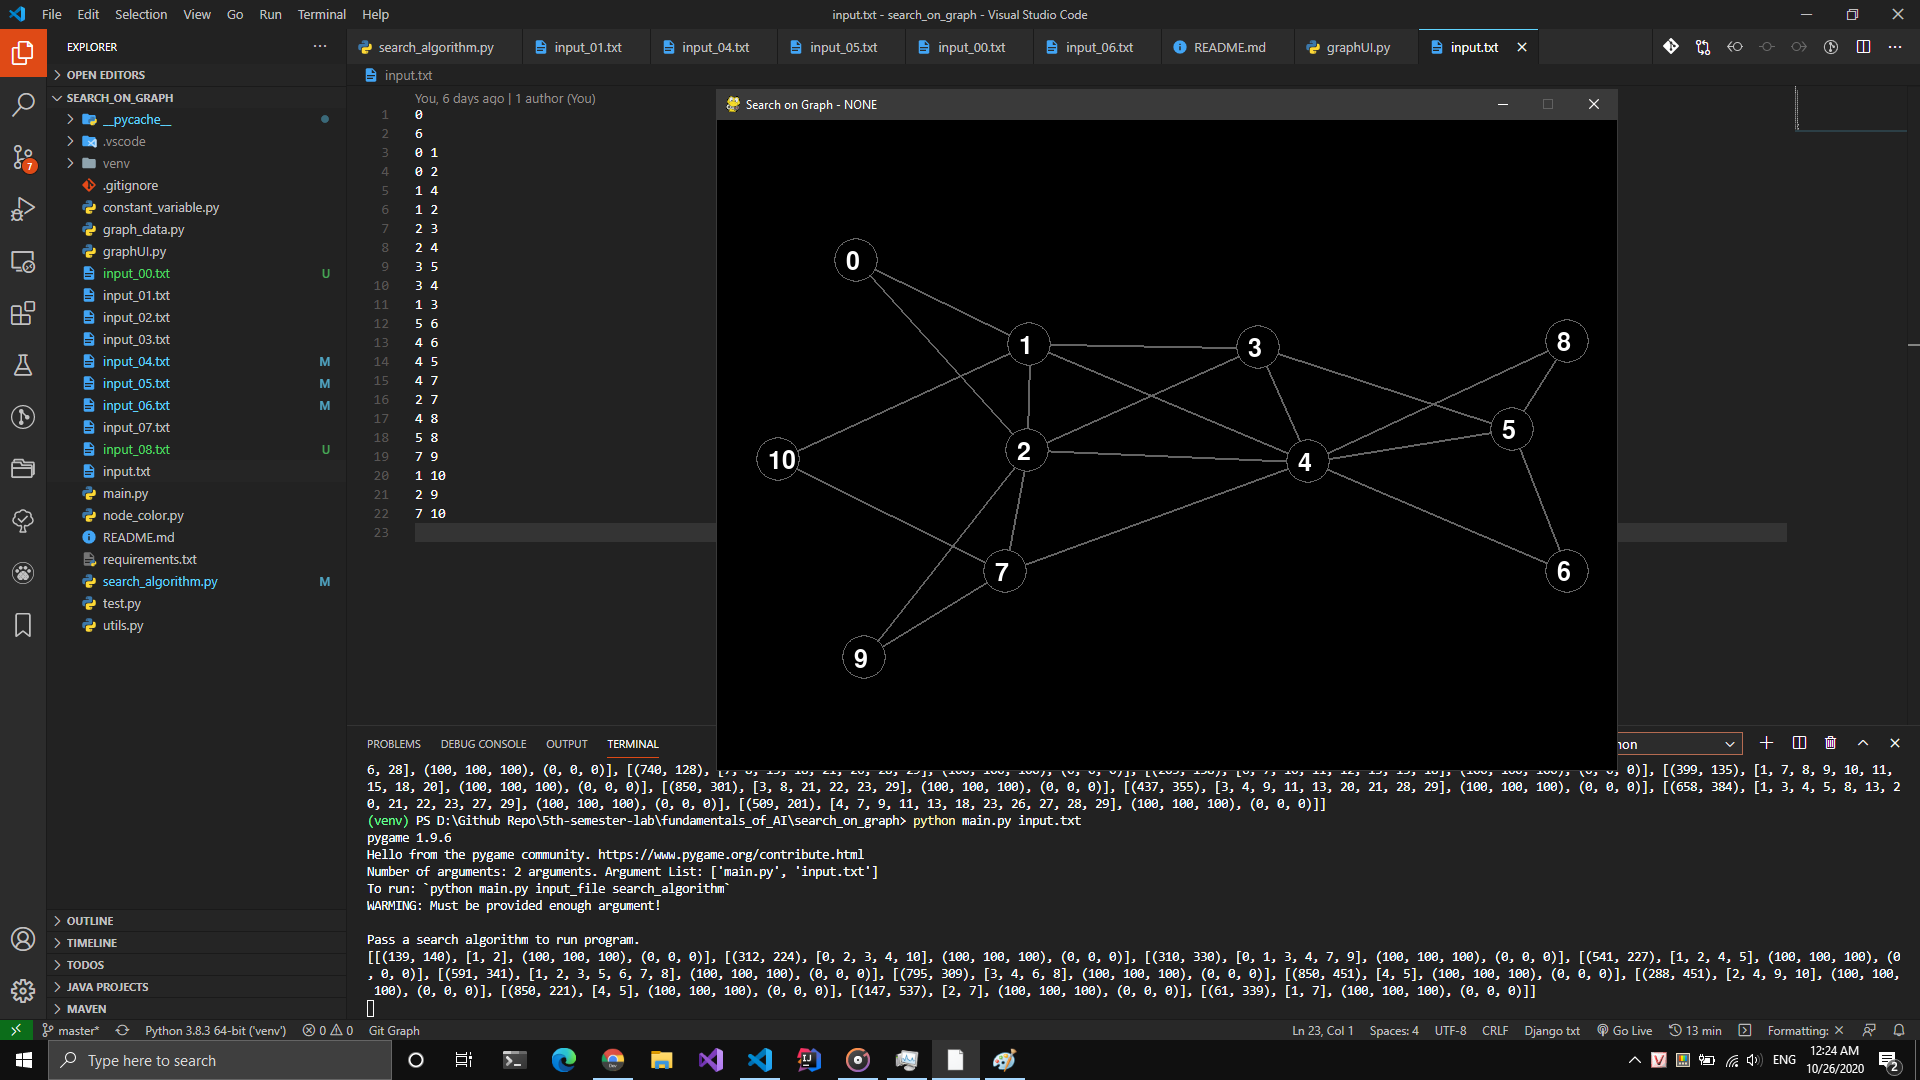
\includegraphics[width=0.98\textwidth]{Test_Case_00_Content.png}
\caption{Testcase mẫu - Test hình dạng đồ thị}
\end{figure}
\subsubsection{Test case 00: File input\_00.txt}
\begin{figure}[H]
\centering
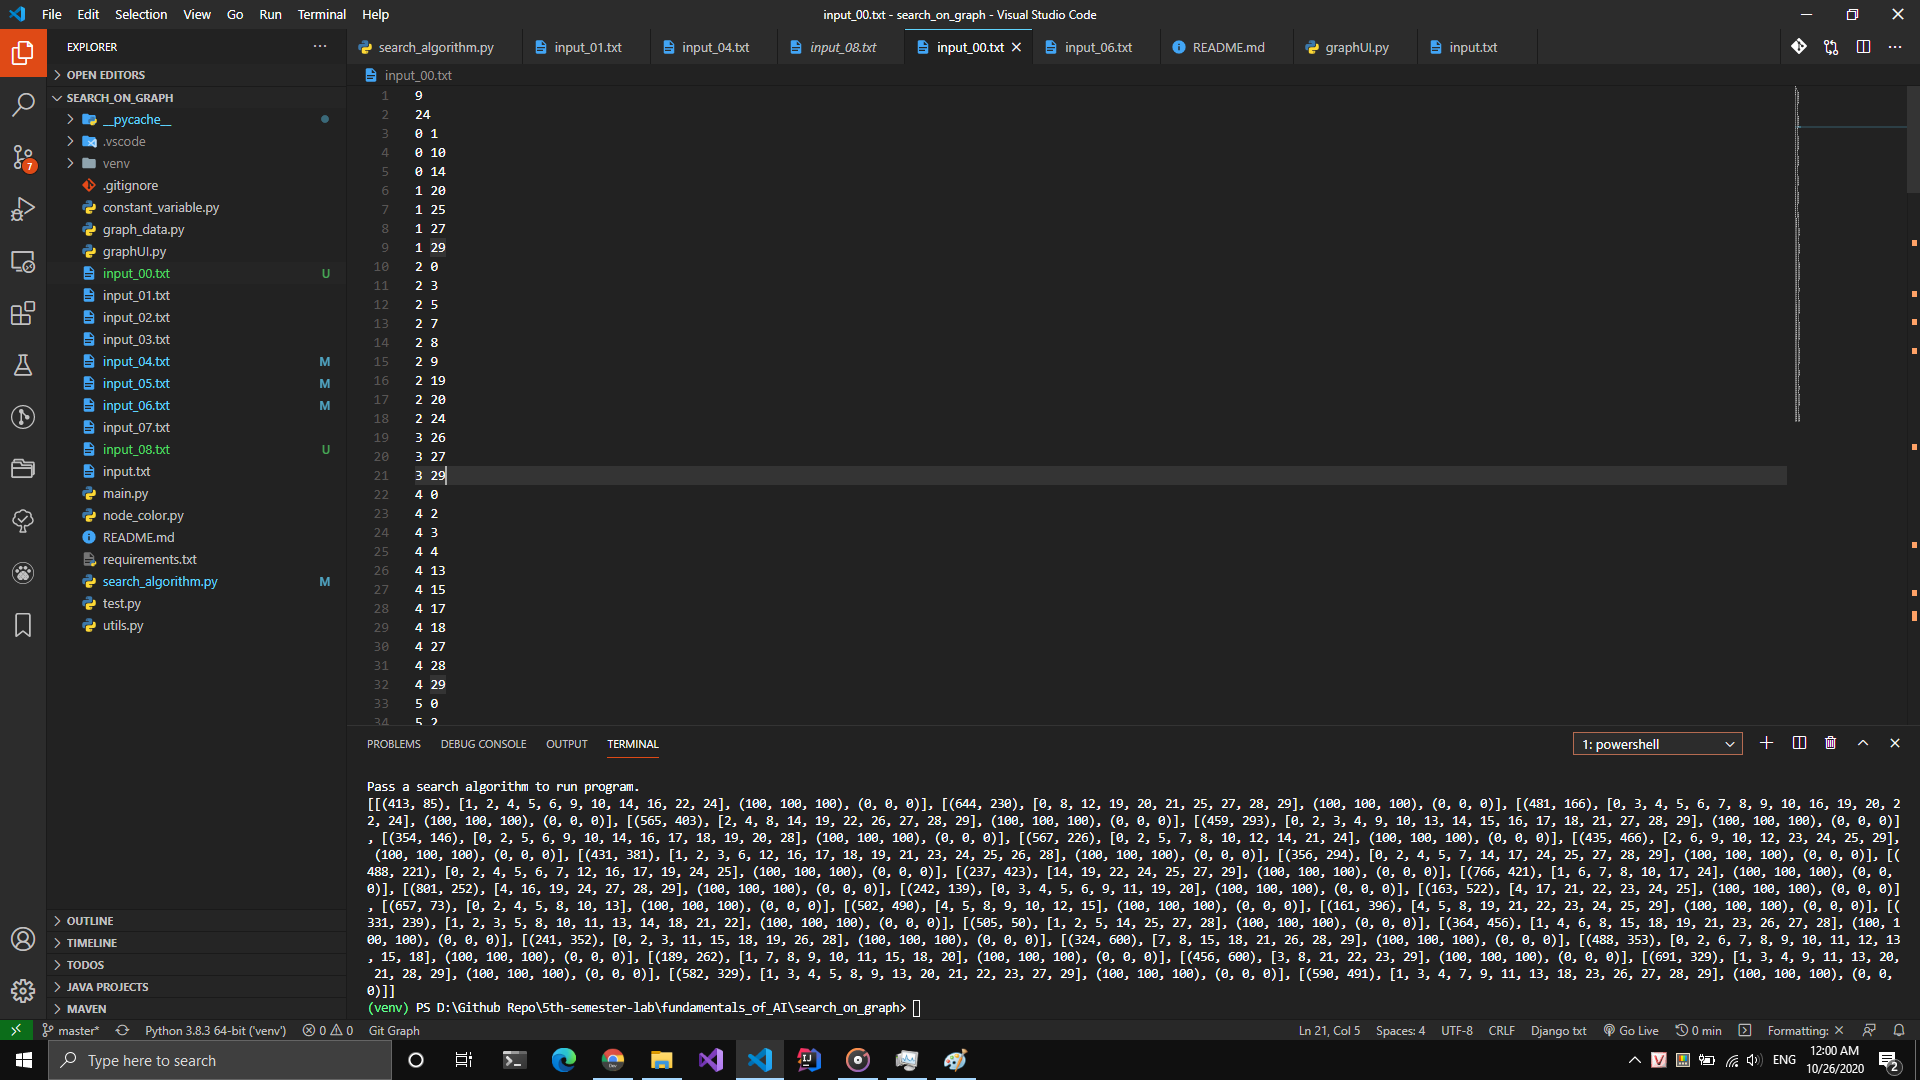
\includegraphics[width=0.5\textwidth]{Test_Case_0.png}
\caption{Testcase 00}
\end{figure}
\begin{figure}[H]
\centering
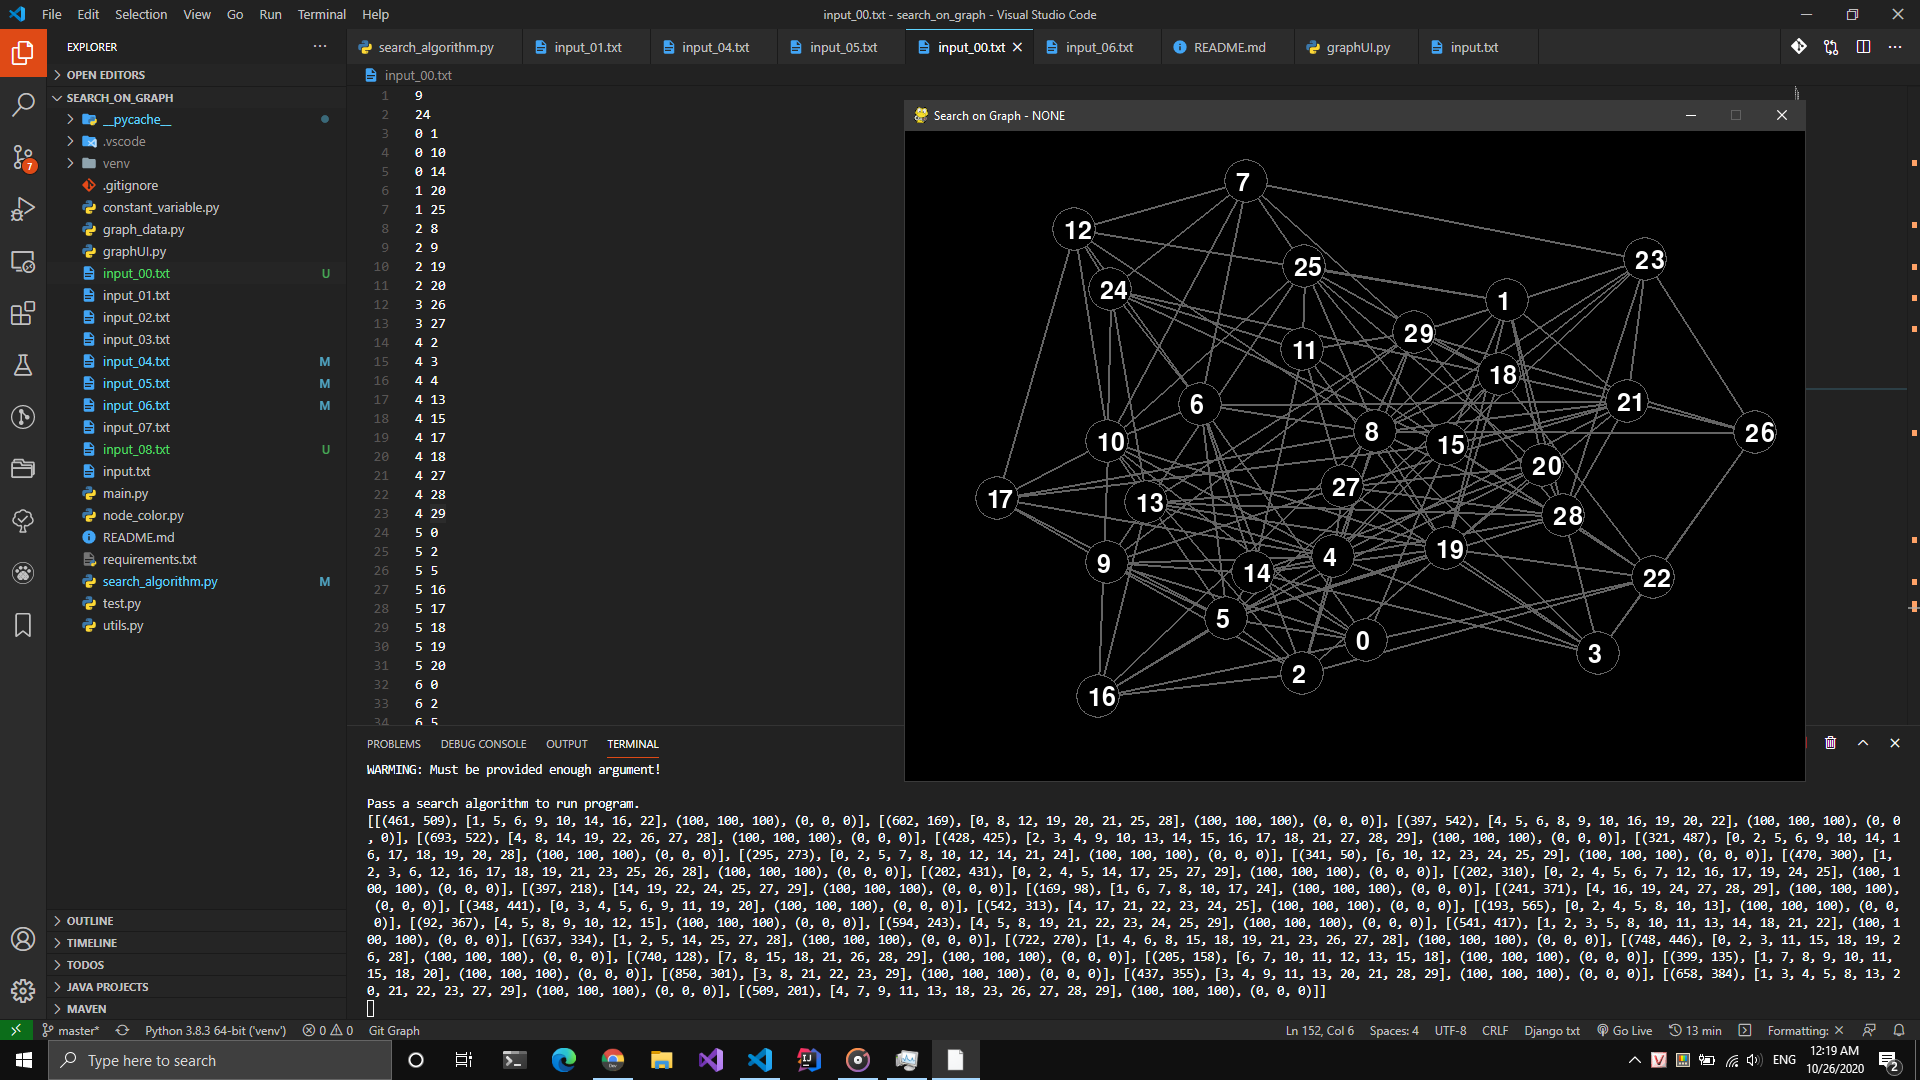
\includegraphics[width=0.98\textwidth]{Test_Case_0_Content.png}
\caption{Testcase 00 - Kích thước 20 đỉnh - Test hình dạng đồ thị}
\end{figure}
\subsubsection{Test case 01: File input\_01.txt}
\begin{figure}[H]
\centering
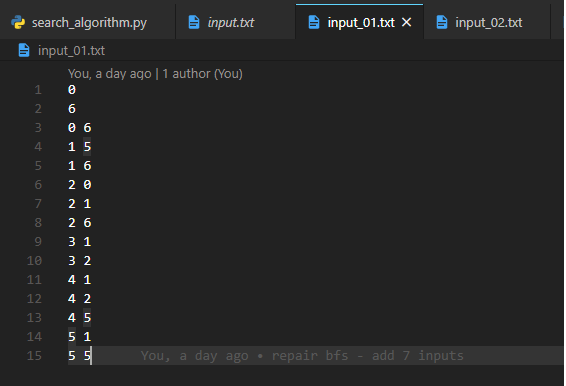
\includegraphics[width=0.5\textwidth]{Test_Case_01_Content.png}
\caption{Testcase 01}
\end{figure}
\begin{figure}[H]
\centering
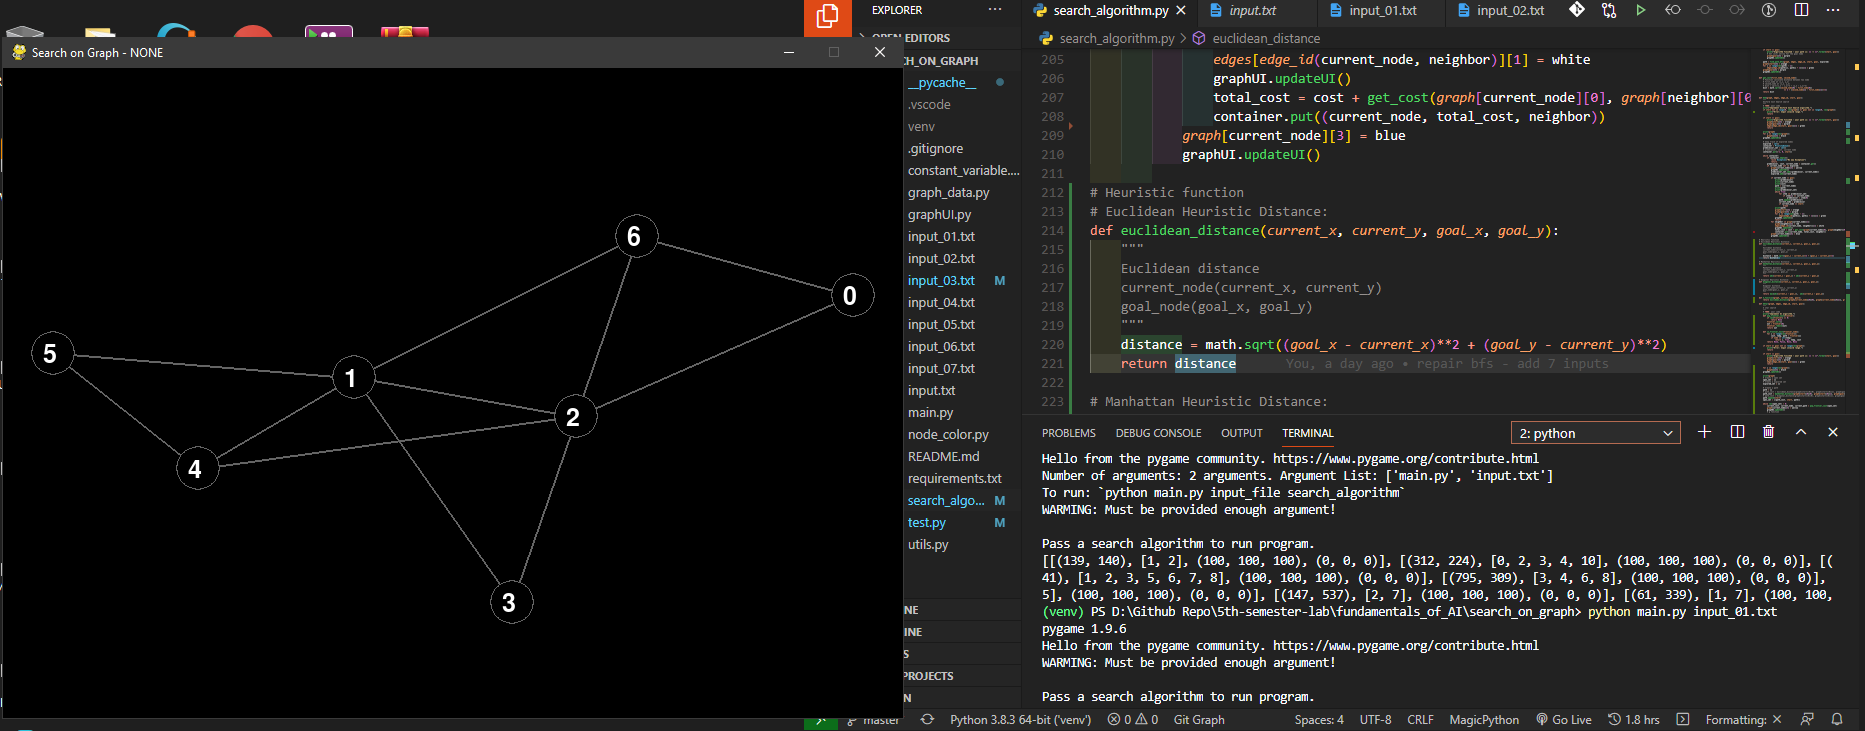
\includegraphics[width=0.98\textwidth]{Test_Case_01.png}
\caption{Testcase 01 - Kích thước 7 đỉnh - Test hình dạng đồ thị}
\end{figure}
\subsubsection{Test case 02: File input\_02.txt}
\begin{figure}[H]
\centering
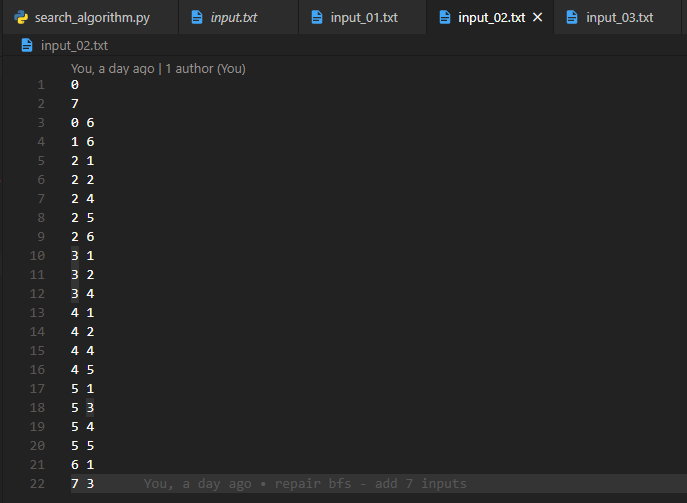
\includegraphics[width=0.5\textwidth]{Test_Case_02_Content.png}
\caption{Testcase 02}
\end{figure}
\begin{figure}[H]
\centering
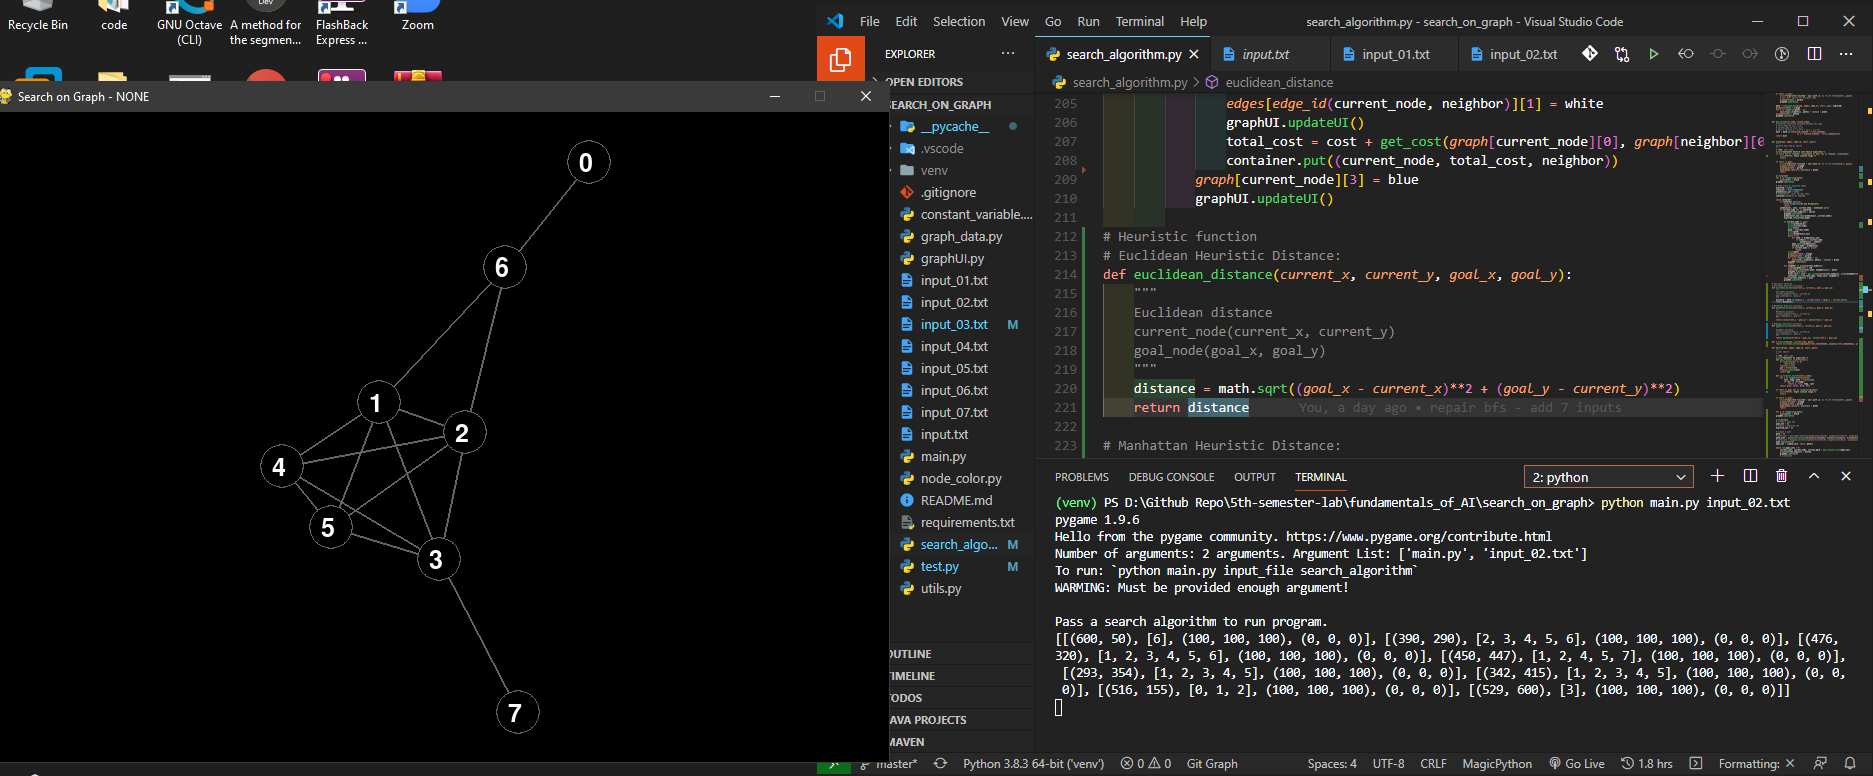
\includegraphics[width=0.98\textwidth]{Test_Case_02.png}
\caption{Testcase 02 - Kích thước 8 đỉnh - Test hình dạng đồ thị}
\end{figure}
\subsubsection{Test case 03: File input\_03.txt}
\begin{figure}[H]
\centering
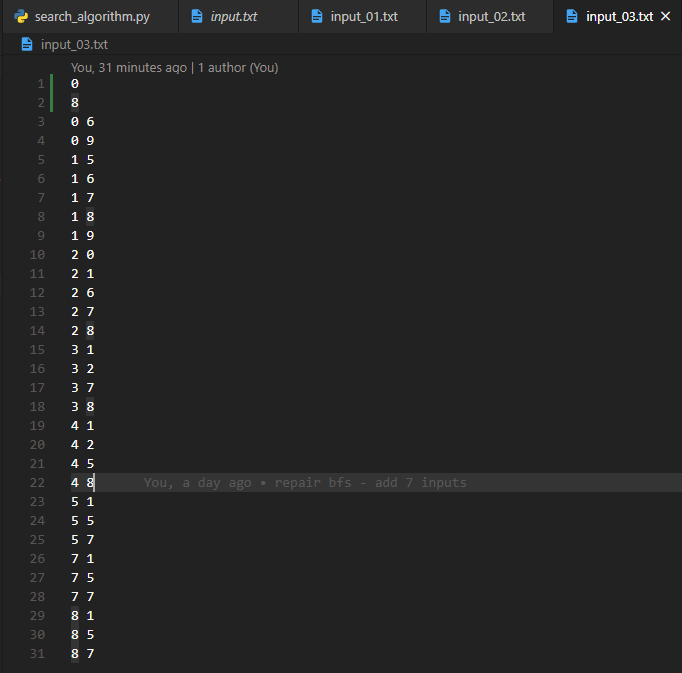
\includegraphics[width=0.5\textwidth]{Test_Case_03_Content.png}
\caption{Testcase 03}
\end{figure}
\begin{figure}[H]
\centering
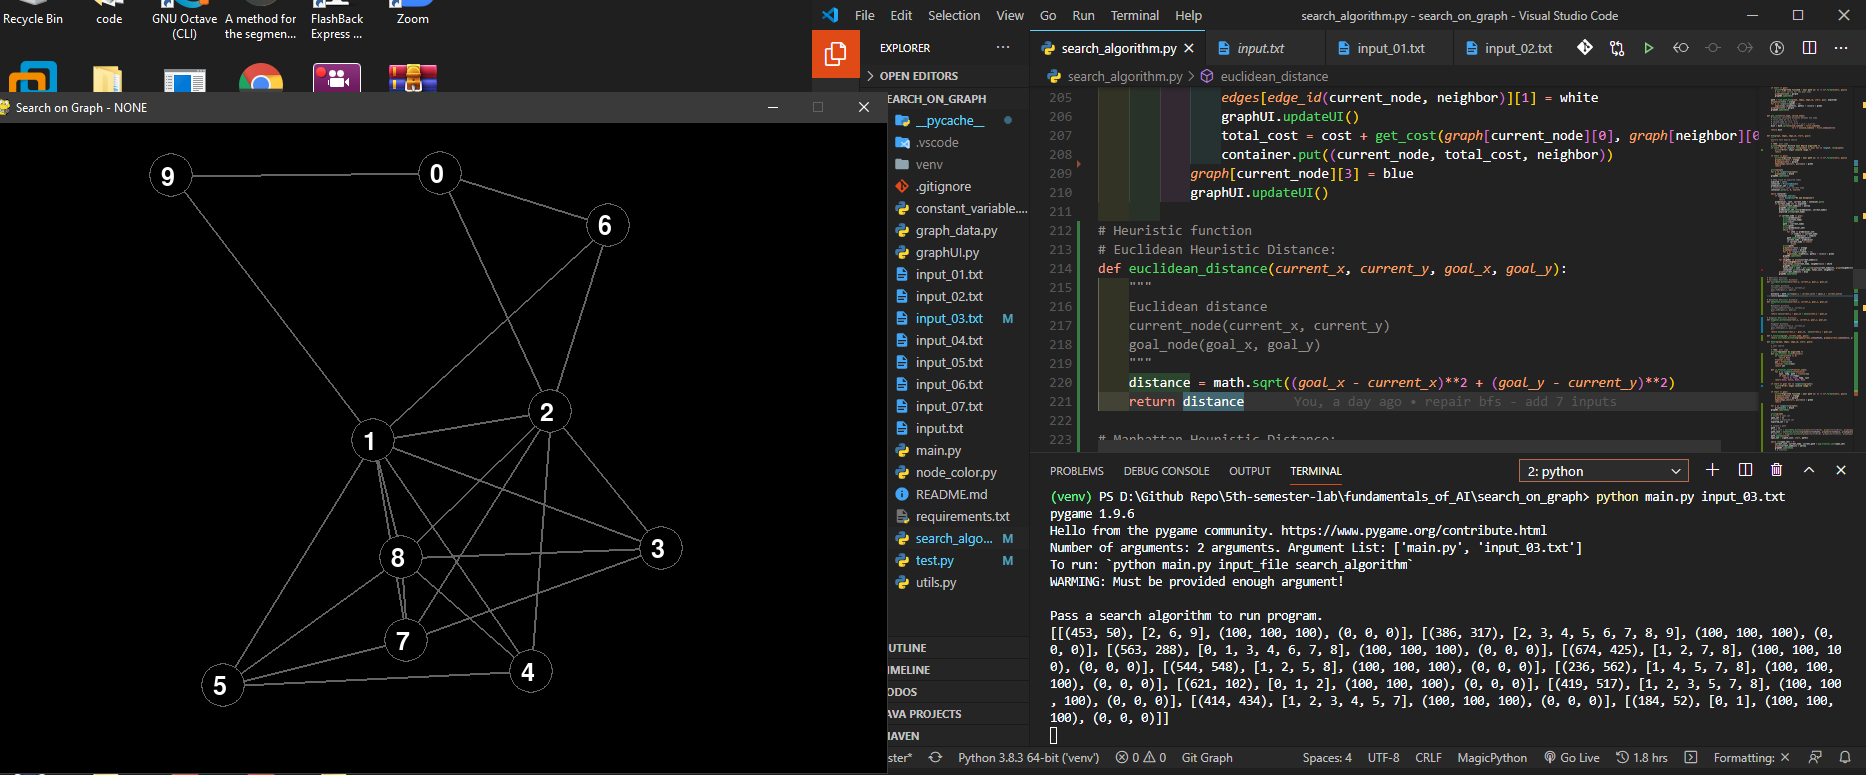
\includegraphics[width=0.98\textwidth]{Test_Case_03.png}
\caption{Testcase 03 - Kích thước 10 đỉnh - Test hình dạng đồ thị}
\end{figure}
\subsubsection{Test case 04: File input\_04.txt}
\begin{figure}[H]
\centering
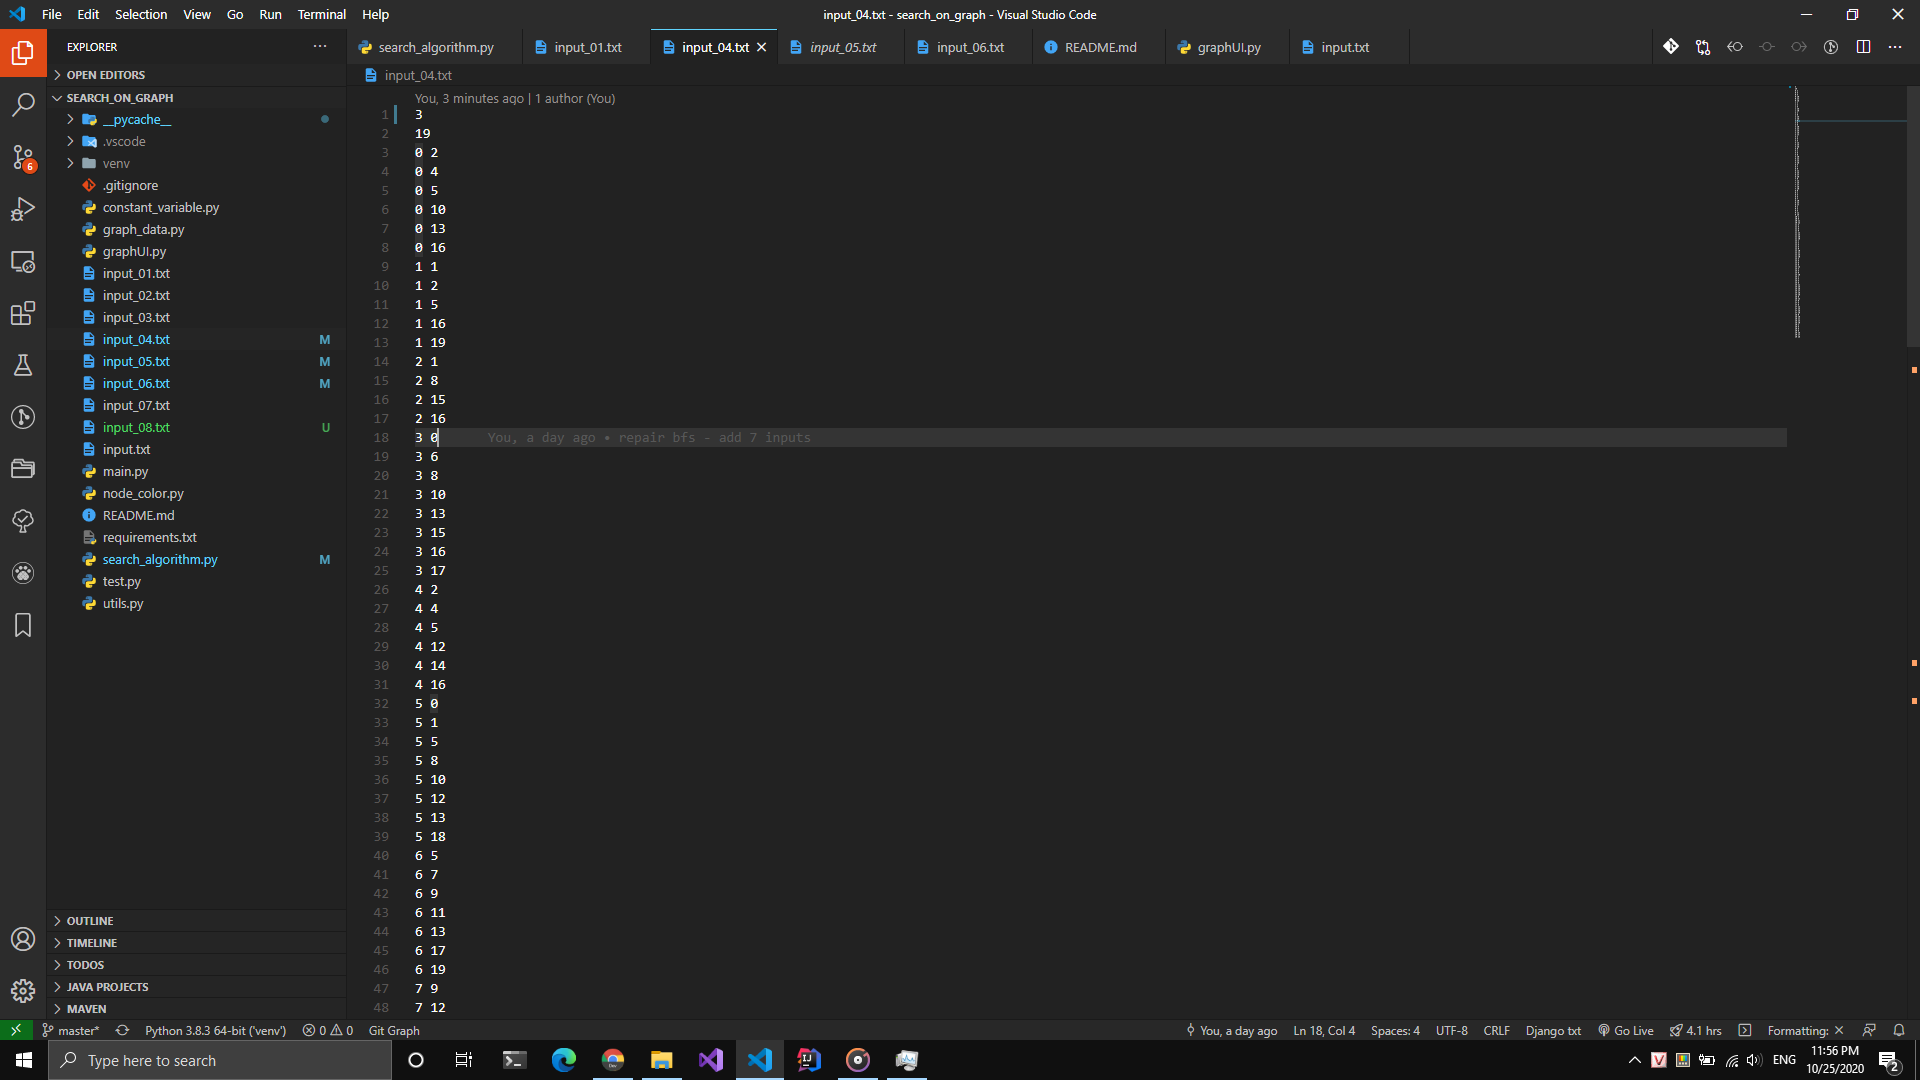
\includegraphics[width=0.5\textwidth]{Test_Case_04.png}
\caption{Testcase 04}
\end{figure}
\begin{figure}[H]
\centering
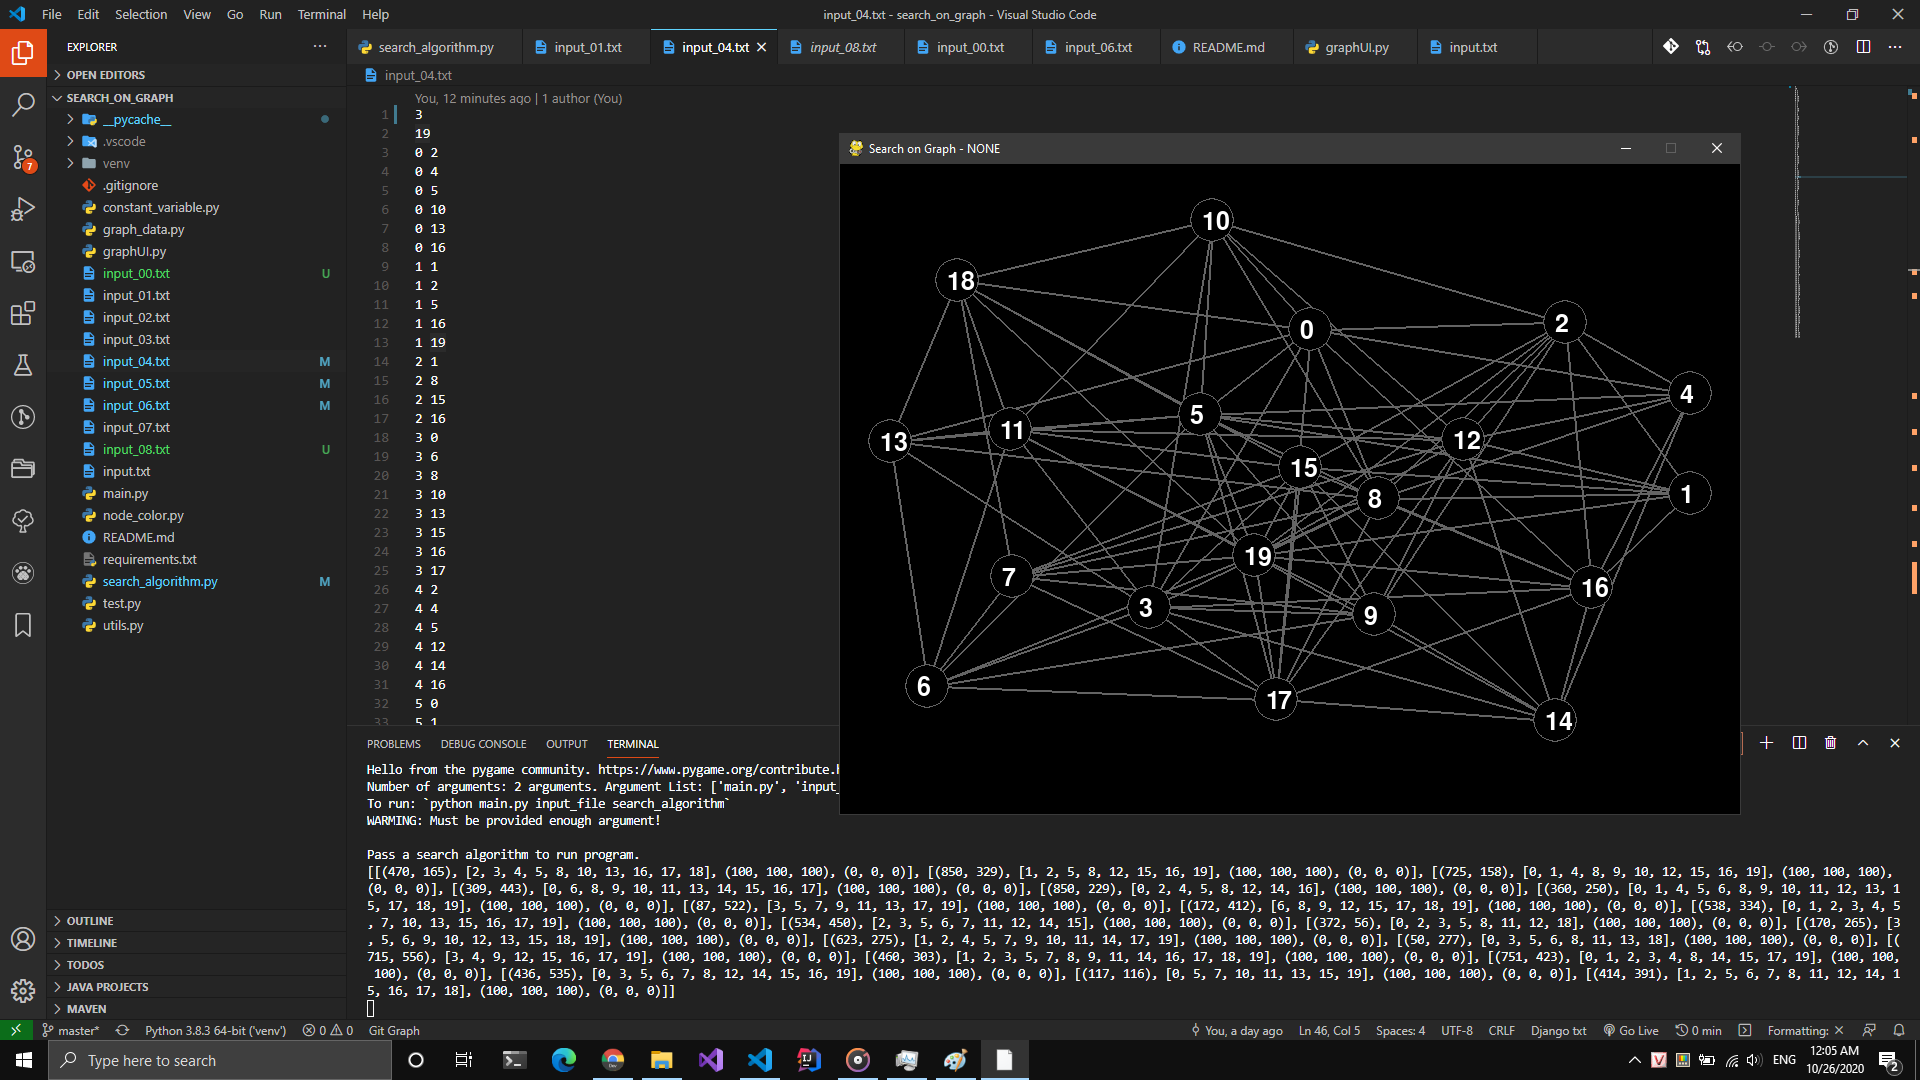
\includegraphics[width=0.98\textwidth]{Test_Case_04_Content.png}
\caption{Testcase 04 - Kích thước 20 đỉnh - Test hình dạng đồ thị}
\end{figure}

Các video kiểm thử với từng thuật toán BFS, DFS, UCS, A Star, Greedy Best-First Search chứa trong thư mục video của đồ án

\newpage

\section{Tài liệu tham khảo}
[1] Lê Hoài Bắc, Tô Hoài Việt. Giáo trình Cơ sở Trí tuệ Nhân tạo. Nhà xuất bản Khoa học và Kỹ thuật. Khoa Công nghệ Thông tin, Trường Đại học Khoa học Tự nhiên, Đại học Quốc gia Tp. Hồ Chí Minh.\newline
[2] Stuart J. Russell and Peter Norvig. Artificial Intelligence: A Modern Approach. (Third Edition). 2010. Publisher Prentice Hall\newline
[3] \href{https://github.com/TheAlgorithms/Python}{Github: TheAlgorithms/Python}
\newpage

\end{document}
